\documentclass[fleqn, 12pt]{article}
\usepackage[a4paper, margin = 21mm]{geometry}
\usepackage[spanish]{babel}
\usepackage{parskip}
\usepackage{amsmath, amsfonts, amsthm}
\usepackage{enumerate}
\usepackage{graphicx}
\usepackage[p,osf]{scholax}
% T1 and textcomp are loaded by package. Change that here, if you want
% load sans and typewriter packages here, if needed
%\usepackage{amsmath,amsthm} must be loaded before newtxmath
% amssymb should not be loaded
\usepackage[scaled=1.075,ncf,vvarbb]{newtxmath}% need to scale up math package
% vvarbb selects the STIX version of blackboard bold.
\newcommand{\derivadaparcial}[2]{\dfrac{\partial {#1}}{\partial {#2}}}
\newcommand{\talque}{\; \middle | \;}

\begin{document}
    \begin{center}
        UNIVERSIDAD AUTÓNOMA DEL ESTADO DE MÉXICO \\
        FACULTAD DE CIENCIAS \\
        DEPARTEMENTO DE MATEMÁTICAS \\
        Cálculo Diferencial Vectorial \\
        Profesores: Dr. Félix Capulín Pérez \\
        Dr. Enrique Castañeda Alvarado \\
        Tarea: Máximos y mínimos
    \end{center}

    Nombre: Osmar Dominique Santana Reyes \hfill No. de cuenta: $ 2125197 $

    \textbf{Instrucciones:} Resuelve cada uno de los ejercicios, justica cada respuesta.

    \begin{enumerate}[\bfseries Ejerc{i}c{i}o 1.]
%-------Ejercicio 1---------------------------------------------------------------------------------------------------
        \item Encontrar los valores máximos y mínimos locales, asi como los puntos silla de las funciones siguientes, después usar un software graficador en tres dimensiones y grafica las funciones teniendo en cuenta que se visualicen todos los aspectos importantes de la función correspondiente.
        
        \begin{enumerate}
%-----------Inciso a) del Ejercicio 1---------------------------------------------------------------------------------
            \item $ f(x,y) = 1 + 2xy - x^2 - y^2 $.
            
            \textbf{Solución.}

            Calculando los puntos críticos de la función:

            $ \derivadaparcial{f}{x} = 2y - 2x = 0 \quad $ y $ \quad \derivadaparcial{f}{y} = 2x - 2y = 0 $

            $ \Longrightarrow 2y - 2x = 0 \quad $ y $ \quad 2x - 2y = 0 $

            $ \Longrightarrow y = x $

            Asi, el conjunto $ A = \left\lbrace (x,y) \in \mathbb{R}^2 \talque x = y \right\rbrace $ contiene a todos los puntos críticos de la función $ f $.

            Luego, se sabe que

            $ 0 \leq (x - y)^2 = x^2 - 2xy + y^2 $

            $ \Longrightarrow 2xy - x^2 - y^2 \leq 0 $

            $ \Longrightarrow 1 + 2xy - x^2 - y^2 \leq 1 $

            Pero si $ (x,y) \in A $ entonces

            $ f(x,y) = 1 + 2xx - x^2 - x^2 = 1 $

            Por lo tanto, $ f $ alcanza su máximo absoluto en los puntos del conjunto $ A $.

            \begin{figure}[h]
                \centering
                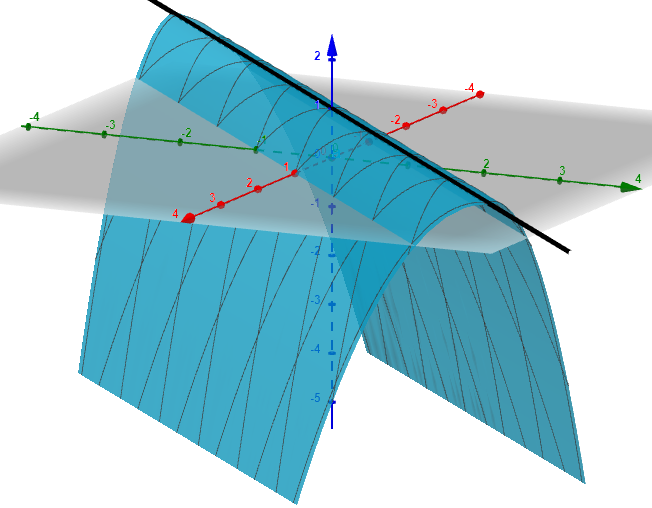
\includegraphics[height = 5cm]{Primero.png}
            \end{figure}

%-----------Inciso b) del Ejercicio 1---------------------------------------------------------------------------------
            \item $ f(x,y) = xy - 2x - 2y $.
            
            \textbf{Solución.}

            Calculando los puntos críticos de la función:

            $ \derivadaparcial{f}{x} = y - 2 = 0 \quad $ y $ \quad \derivadaparcial{f}{y} = x - 2 = 0 $

            $ \Longrightarrow y - 2 = 0 \quad $ y $ \quad x - 2 = 0 $

            $ \Longrightarrow y = 2 \quad $ y $ \quad x = 2 $

            Asi, $ (2,2) $ es un punto crítico de $ f $.

            Si $ y = x $ entonces $ f(x,y) = x^2 - 4x $, el cual alcanza su mínimo en $ x = 2 $.

            Si $ y = 4 - x $ entonces $ f(x,y) = x(4-x) - 2x - 2(4-x) = 4x - x^2 - 8 $, el cual alcanza su máximo en $ x = 2 $.

            Por lo tanto, $ (2,2) $ es un punto silla de $ f $.

            \begin{figure}[h]
                \centering
                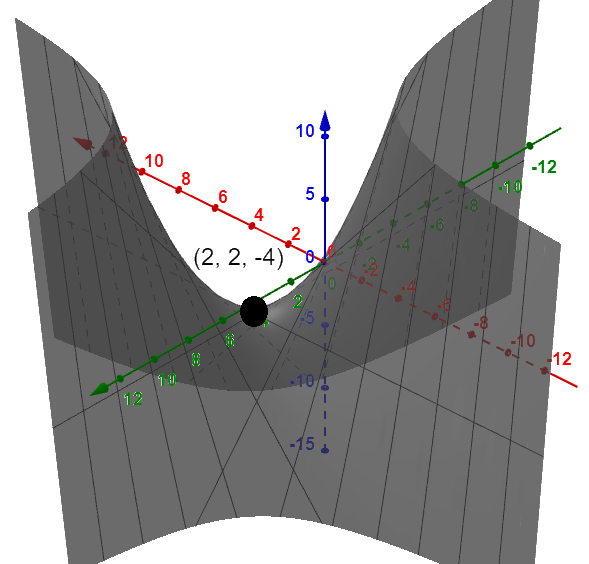
\includegraphics[height = 7cm]{Segundo.png}
            \end{figure}

%-----------Inciso c) del Ejercicio 1---------------------------------------------------------------------------------
            \item $ f(x,y) = \dfrac{x^2 y^2 - 8x + y}{xy} $.
            
            \textbf{Solución.}

            Calculando los puntos críticos de la función:

            $ \derivadaparcial{f}{x} = \dfrac{(xy)(2x y^2 - 8) - (x^2 y^2 - 8x + y)(y)}{x^2 y^2} = 0 \quad $ y

            $ \derivadaparcial{f}{y} = \dfrac{(xy)(2x^2 y + 1) - (x^2 y^2 - 8x + y)(x)}{x^2 y^2} = 0 $


            $ \Longrightarrow (xy)(2x y^2 - 8) - (x^2 y^2 - 8x + y)(y) = 0 \quad $ y

            \hspace{7mm} $ (xy)(2x^2 y + 1) - (x^2 y^2 - 8x + y)(x) = 0 $


            $ \Longrightarrow 2x^2 y^3 - 8xy - x^2 y^3 + 8xy - y^2 = 0 \quad $ y

            \hspace{7mm} $ 2x^3 y^2 + xy - x^3 y^2 + 8x^2 - xy = 0 $


            $ \Longrightarrow x^2 y^3 - y^2 = 0 \quad $ y $ \quad x^3 y^2 + 8x^2 = 0 $

            $ \Longrightarrow y^2(x^2 y - 1) = 0 \quad $ y $ \quad x^2(xy^2 + 8) = 0 $

            $ \Longrightarrow x = 0, \quad y = 0 \quad $ y se tiene el siguiente sistema de ecuaciones
            \begin{align}
                x^2 y - 1 = 0 \label{eq:1c1} \\
                xy^2 + 8 = 0 \label{eq:1c2}
            \end{align}
            De (\ref{eq:1c1}) se tiene que $ y = \dfrac{1}{x^2} $. Sustituyendo esto en (\ref{eq:1c2}), se tiene que

            $ x \left( \dfrac{1}{x^2} \right)^2 + 8 = 0 $

            $ \Longrightarrow \dfrac{1}{x^3} = -8 $

            $ \Longrightarrow x^3 = -\dfrac{1}{8} $

            $ \Longrightarrow x = -\dfrac{1}{2} $

            Sustituyendo en (\ref{eq:1c1}): 

            $ \left( -\dfrac{1}{2} \right)^2 y - 1 = 0 $

            $ \Longrightarrow \dfrac{y}{4} = 1 $

            $ \Longrightarrow y = 4 $

            Pero $ (0,0) $ no pertenece al dominio de $ f $, pues $ f(0,0) = \dfrac{0}{0} $, por lo que no es un punto crítico.

            Así, $ \left( -\dfrac{1}{2}, 4 \right) $ es un punto crítico de $ f $.

%-----------Inciso d) del Ejercicio 1---------------------------------------------------------------------------------
            \item $ f(x,y) = e^x \cos (y) $.
            
            \textbf{Solución.}

            Calculando los puntos críticos de la función:

            $ \derivadaparcial{f}{x} = e^x \cos (y) = 0 \quad $ y $ \derivadaparcial{f}{y} = -e^x \sen (y) = 0 $

            $ \Longrightarrow e^x \cos (y) = 0 \quad $ y $ \quad -e^x \sen (y) = 0 $

            $ \Longrightarrow \cos (y) = 0 \quad $ y $ \quad - \sen (y) = 0 $

            $ \Longrightarrow y = k \, \dfrac{\pi}{2} $ con $ k \in \mathbb{N} $

            \begin{figure}[h!]
                \centering
                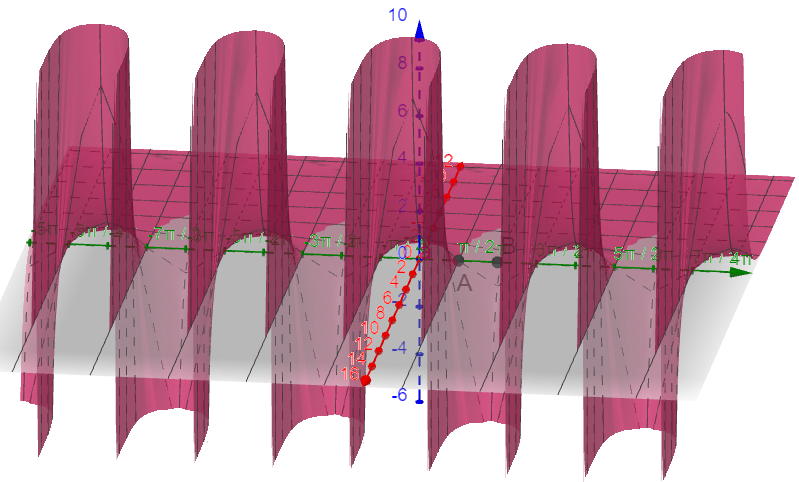
\includegraphics[height = 5cm]{Cuarto.png}
            \end{figure}

            Asi, el conjunto $ B = \left\lbrace (x,y) \in \mathbb{R}^2 \talque y = k \, \dfrac{\pi}{2} \text{ con } k \in \mathbb{N} \right\rbrace $ contiene a todos los puntos críticos de la función $ f $.

            Luego, se sabe que $ 0 < e^x < \infty $ y $ -1 \leq \cos (y) \leq 1 $. Si $ -1 \leq \cos (y) < 0 $ entonces $ - \infty < e^x \cos (y) < 0 $. Y si $ 0 < \cos (y) \leq 1 $ entonces $ 0 < e^x cos(y) < \infty $. De esta manera, $ - \infty < e^x \cos (y) < \infty $. Por lo tanto, $ f $ no tine máximos ni mínimos locales y los puntos del conjunto $ B $ son puntos silla.

%-----------Inciso e) del Ejercicio 1---------------------------------------------------------------------------------
            \item $ f(x,y) = x \sen (y) $.
            
            \textbf{Solución.}

            Calculando los puntos críticos de la función:

            $ \derivadaparcial{f}{x} = \sen (y) = 0 \quad $ y $ \quad \derivadaparcial{f}{y} = x \cos (y) = 0 $

            $ \Longrightarrow \sen (y) = 0 \quad $ y $ \quad x \cos (y) = 0 $

            $ \Longrightarrow y = k \pi \text{ con } k \in \mathbb{N} \quad $ y $ \quad x \cos (y) = 0 $

            $ \Longrightarrow y = k \pi \text{ con } k \in \mathbb{N} \quad $ y $ \quad x \lvert 1 \rvert = 0 $

            $ \Longrightarrow y = k \pi \text{ con } k \in \mathbb{N} \quad $ y $ \quad x = 0 $

            Asi, el conjunto $ C = \left\lbrace (x,y) \in \mathbb{R}^2 \talque x = 0, y = k \pi \text{ con } k \in \mathbb{N} \right\rbrace $ contiene a todos los puntos críticos de la función $ f $.

            Ahora, si $ y = \dfrac{\pi}{2} $ entonces $ f(x,y) = x $ y como $ - \infty \leq x \leq \infty $ entonces $ f $ no tiene ningún extremo local en $ x = 0 $. 
            
            Por lo tanto, los puntos del conjunto $ C $ son puntos silla.

            \begin{figure}[h]
                \centering
                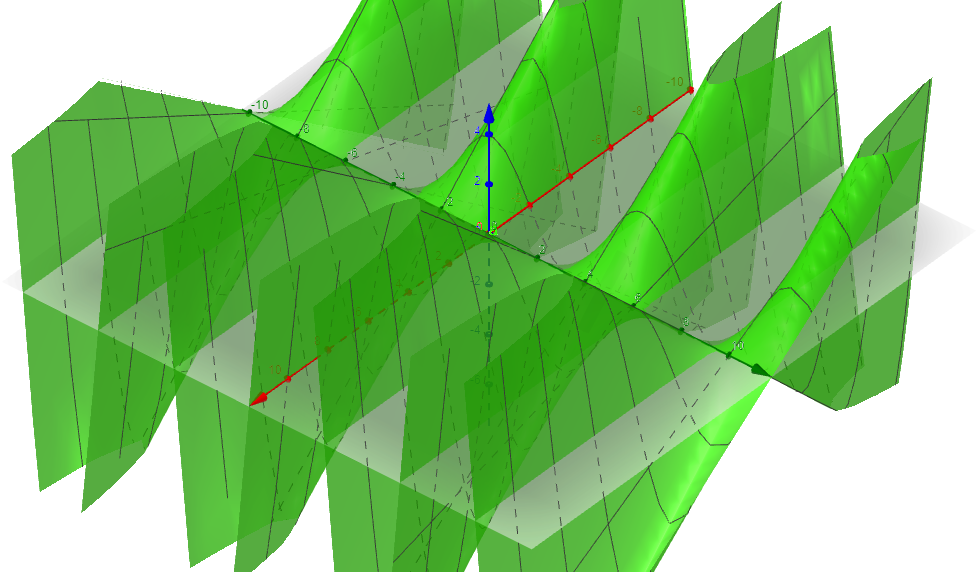
\includegraphics[height = 5cm]{Quinto.png}
            \end{figure}

        \end{enumerate}

%-------Ejercicio 2---------------------------------------------------------------------------------------------------
        \item Encontrar los valores máximo y mínimo absolutos de $ f $ en la región $ D $.
        
        \begin{enumerate}
%-----------Inciso a) del Ejercicio 2---------------------------------------------------------------------------------
            \item $ f(x,y) = x^2 + y^2 + x^2 y + 4, \, D = \left\lbrace (x,y) \in \mathbb{R}^2 : \lvert x \rvert \leq 1, \lvert y \rvert \leq 1 \right\rbrace $.
            
            \textbf{Solución.}

            Sea $ (x,y) \in D $ entonces $ \lvert x \rvert \leq 1 \quad $ y $ \quad \lvert y \rvert \leq 1 $

            $ \Longrightarrow -1 \leq x \leq 1 \quad $ y $ \quad -1 \leq y \leq 1 $

            $ \Longrightarrow 0 \leq x^2 \leq 1 \quad $ y $ \quad 0 \leq y^2 \leq 1 $

            $ \Longrightarrow 0 \leq x^2 \leq 1 $, $ \quad 0 \leq y^2 \leq 1 \quad $ y $ \quad 0 \leq x^2 y \leq 1 $

            $ \Longrightarrow 4 \leq x^2 + y^2 + x^2 y + 4 \leq 1 + 1 + 1 + 4 = 7 $

            De esta forma, $ f $ está acotada entre 4 y 7. Luego, notemos que 
            
            $ f(0,0) = 0^2 + 0^2 + 0^2 (0) + 4 = 4 \quad $ y 
            
            $ f(1,1) = 1^2 + 1^2 + 1^2 (1) + 4 = 7 = (-1)^2 + 1^2 + (-1)^2 (1) + 4 = f(-1,1) $.

            Por lo tanto, $ f $ alcanza su mínimo absoluto en $ (0,0) $ y su máximo absoluto en $ (-1,1) $ y $ (1,1) $.

%-----------Inciso b) del Ejercicio 2---------------------------------------------------------------------------------
            \item $ f(x,y) = 1 + xy - x - y, \, D $ es la región acotada por la parábola $ y = x^2 $ y la recta $ y = 4 $.
            

%-----------Inciso c) del Ejercicio 2---------------------------------------------------------------------------------
            \item $ f(x,y) = 2x^3 + y^4, \, D = \left\lbrace (x,y) \in \mathbb{R}^2 : x^2 + y^2 \leq 1 \right\rbrace $.
            
        \end{enumerate}
%-------Ejercicio 3---------------------------------------------------------------------------------------------------
        \item Encontrar el punto del plano $ 2x - y + z = 1 $ que sea más cercano al punto $ (-4,1,3) $.

        \textbf{Solución.}
        
        Sea $ (x,y,z) $ un punto del plano $ 2x - y + z = 1 $ entonces la distancia entre este punto y el punto $ (-4,1,3) $ esta dada por 

        $ \sqrt{(x + 4)^2 + (y - 1)^2 + (z - 3)^2} $

        Luego, de la ecuación del plano $ 2x - y + z = 1 $ se tiene que $ z = 1 + y - 2x $. Sustituyendo esto en la expresión anterior se tiene que

        $ \sqrt{(x + 4)^2 + (y - 1)^2 + (1 + y - 2x - 3)^2} = \sqrt{(x + 4)^2 + (y - 1)^2 + (y - 2x - 2)^2} $

        Como la raíz cuadrada es una función creciente entonces basta con encontrar el mínimo absoluto de $ (x + 4)^2 + (y - 1)^2 + (y - 2x - 2)^2 $.

        Así, sea $ g(x,y) = (x + 4)^2 + (y - 1)^2 + (y - 2x - 2)^2 $. Calculando los puntos críticos de la función, se tiene que

        $ \derivadaparcial{g}{x} = 2(x + 4) - 4(y - 2x - 2) = 0 \quad $ y $ \quad \derivadaparcial{g}{y} = 2(y - 1) + 2(y - 2x - 2) = 0 $

        $ \Longrightarrow 2(x + 4) - 4(y - 2x - 2) = 0 \quad $ y $ \quad 2(y - 1) + 2(y - 2x - 2) = 0 $

        $ \Longrightarrow 2x + 8 - 4y + 8x + 8 = 0 \quad $ y $ \quad 2y - 2 + 2y - 4x - 4 = 0 $

        $ \Longrightarrow 10x - 4y + 16 = 0 \quad $ y $ \quad -4x + 4y - 6 = 0 $

        De esta manera, se forma el siguiente sistema de ecuaciones
        \begin{align}
            10x - 4y = -16 \label{eq:41} \\
            -4x + 4y = 6 \label{eq:42}
        \end{align}
        Sumando (\ref{eq:41}) y (\ref{eq:42}): $ 6x = -10 \Longrightarrow x = -\dfrac{5}{3} $. Sustituyendo en (\ref{eq:42}) se tiene que $ -4 \left( -\dfrac{5}{3} \right) + 4y = 6 \Longrightarrow 4y = 6 - \dfrac{20}{3} \Longrightarrow y = -\dfrac{2}{12} = -\dfrac{1}{6} $

        Por lo tanto, $ \left( -\dfrac{5}{3}, -\dfrac{1}{6} \right) $ es un punto crítico de $ g $.

%-------Ejercicio 4---------------------------------------------------------------------------------------------------
        \item Encontrar el punto de la superficie $ x^2 y^2 z = 1 $ que sea más cercano al origen.
        
        
%-------Ejercicio 5---------------------------------------------------------------------------------------------------
        \item Encontrar tres números positivos cuya suma sea 100 y cuyo producto sea mínimo.
    

%-------Ejercicio 6---------------------------------------------------------------------------------------------------
        \item Encontrar el volumen de la mayor caja rectangular con bordes paralelos a los ejes que pueda estar inscrita en el elipsoide $ 9x^2 + 36y^2 + 4z^2 = 36 $.
        

%-------Ejercicio 7---------------------------------------------------------------------------------------------------
        \item Encontrar las dimensiones de la caja rectangular con máximo volumen y área superficial total de 64 cm$ ^2 $.
        

%-------Ejercicio 8---------------------------------------------------------------------------------------------------
        \item La base de una pecera con volumen $ V $ dado esta hecha de pizarra y, los lados, de vidrio. Si la pizarra cuesta 5 veces (por unidad de área) más que el vidrio encontrar las dimensiones de la pecera que reduzca al mínimo el costo de los materiales.
        

%-------Ejercicio 9---------------------------------------------------------------------------------------------------
        \item Tres alelos (formas mutantes de genes) A, B y O, determinan los cuatro tipos sanguíneos A (AA o AO), B (BB o BO), O (OO) y AB. La ley de Hardy-Weinberg expresa que la proporción de individuos en una población que llevan los alelos diferentes es
        $$ P = 2pq + 2rp + 2rq $$
        donde $ p, q, r $ son las proporciones de $ A, B, O $ en la población. Utilizar el hecho de que $ p + q + r = 1 $ para demostrar que $ P $ es, a lo sumo $ \frac{2}{3} $.


%-------Ejercicio 10--------------------------------------------------------------------------------------------------
        \item Encontrar la ecuación del plano que pasa por el punto (1,2,3) y determina el volumen más pequeño en el primer octante.
        
    \end{enumerate}
\end{document}
